\chapter{Design}\label{C:design}

The design processes outlined within this report will draw heavily on the background research discussed in \Cref{C:background}. These designs aim to effectively implement the outlined system requirements discussed by \Cref{S:goals} in a robust and repeatable manner.


%
% SECTION Defining & Justifying System Specifications
%

\section{System Specifications and Architecture}\label{S:specs_design}

\Cref{S:goals} outlines a list of specifications that this project must achieve. For each item in this list, design specifications can be derived to ensure that our designs are capable of meeting the outlined requirements. This list of specifications will also help to shape the architectural approach taken on this project.


\subsubsection*{Requirement 1: Operate with a 12V DC input supply voltage}

To meet this requirement, the buck converter must be designed to be 12V DC compatible. this will require all designed hardware, including additional digital and analog circuity to be capable of operating with this supply.

\subsubsection*{Requirement 2: Provide a selectable DC output voltage between 3V and 10V}

To meet this requirement, the designed buck converter must have the ability to change the duty cycle of it's PWM switching signal. This will allow for variation of the output voltage based on \Cref{E:V_out}.

\subsubsection*{Requirement 3: Provide an output voltage precision of at least $\pm5\%$ of the targeted output voltage}

To meet this requirement, the designed buck converter must have a control system to regulate the output voltage. To achieve a steady state error of less than $\pm5\%$, feedback should be implemented, requiring output voltage sensing. We can also specify that a minimum duty cycle resolution of 1.25\% will be required to achieve this. For the derivation of these values, please see \Cref{A:specs}.

\subsubsection*{Requirement 4: Provide a selectable inductor current ripple between 20\% and 50\% of the total output current}

To meet this requirement, the designed buck converter must have the ability to change the frequency of it's PWM switching signal. This will allow for variation of the inductor peak to peak current ripple based on equation \Cref*{E:delta_i}. 

\subsubsection*{Requirement 5: Provide a variable converter switching frequency between 1kHz and 100kHz}

To meet this requirement, the PWM switching frequency must be selectable across the specified range. This, in tandem with requirement 4, allow for the specification of the inductor range for which these requirements can be met. For the derivation of these values, please see \Cref{A:specs}.

\subsubsection*{Requirement 6: Provide  an  inductor  current  ripple  precision  of  at  least $\pm$5\%  of  the  target  inductor current ripple}

To meet this requirement, the designed buck converter must have a control system to regulate the inductor current ripple. To achieve a steady state error of $\pm$5\%, feedback should be implemented, requiring inductor current ripple sensing. We can also specify that a minimum frequency selection resolution of 200Hz, as well as a minimum current ripple measurement resolution of a resolution of 15mA will be required to achieve this. For the derivation of these values, please see \Cref{A:specs}.  


\subsubsection*{Requirement 7: Operate with variable load sizes between $10\Omega$ and $20\Omega$}

To meet this requirement, all components of the buck converter must be designed to handle the maximum output current of 1A that will occur with a $10\Omega$ load at 10V. It will also be important that any current sensing is designed to operate within the range defined by these loads. Finally it is required that control systems are implemented to maintain requirements 3, \& 6 as the load varies. 

\subsection{System Architecture}

Based on the specifications outlined in the above section, an architecture that outlines the system design has been developed. This architecture has been divided into three subsystems that must each be developed. This architecture system can be seen in \Cref{F:sys_overview}.\\

Subsystem one implements a PWM generator. From requirements 2, \& 5 it has been identified that a PWM generator capable of varying both the duty cycle and the frequency of it's output signal independently must be designed. This system can be seen in \Cref{F:sys_overview} outlined in green.\\

Subsystem two implements system state sensing. From requirement 3 \& 6 it has been identified that an output voltage sensor, and an inductor current ripple sensor must be designed. This system can be seen in \Cref{F:sys_overview} outlined in blue.\\

Subsystem three implements two control systems. From requirements 3, 6, \& 7 it has been identified that control systems should be designed to ensure that the specified steady state errors of the output voltage and inductor current ripple are met. 

One control system will take the output load voltage measurement, and control the PWM duty cycle. The other control system will take the inductor current ripple, and control the PWM frequency. This system can be seen in \Cref{F:sys_overview} outlined in red.

\newpage

\begin{figure}[!h]
    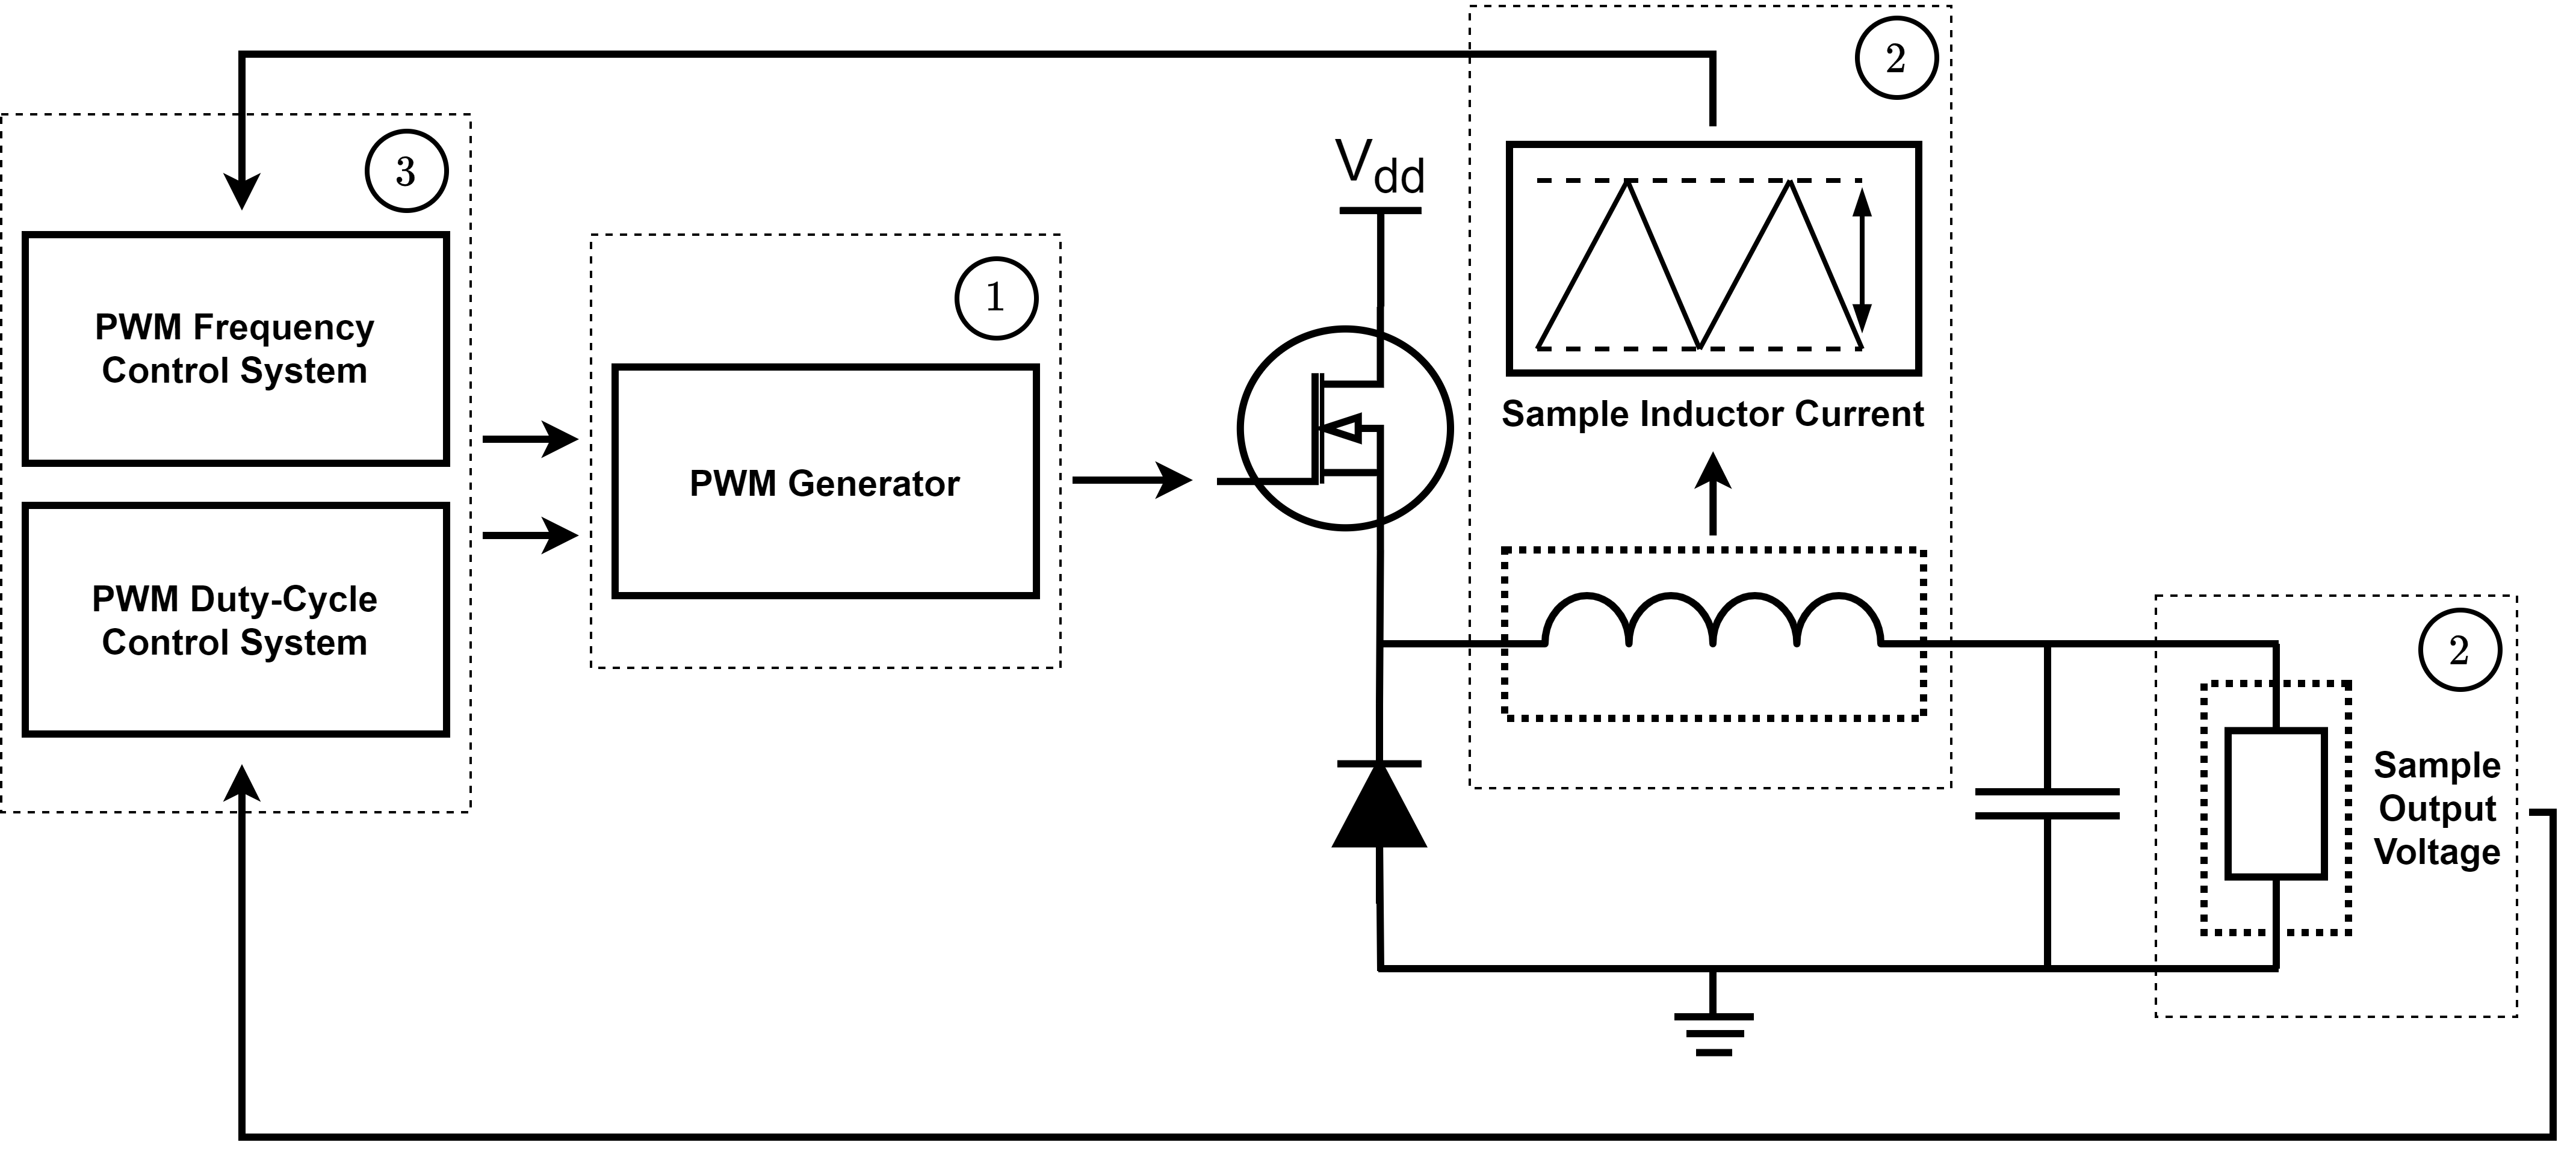
\includegraphics[width = \textwidth]{System_Overview.png}
    \caption{System architecture design, with three internal subsystems}
    \label{F:sys_overview}
\end{figure}


% It has been specified that the final system design will be able to select for both the output load voltage, and the inductor current ripple of the buck converter. From this requirement we can identity that two separate control systems should be designed, one to regulate the output voltage of the converter, and one to regulate the inductor current ripple.

% Next we can identify that to control the output load voltage and the inductor current ripple, we must be able to actively effect their current state. Based on \Cref{E:V_out} we can see that by varying the duty cycle of the converters PWM signal, we are able to directly control the output voltage. Similarly, from \Cref{E:delta_i} we can see that by varying the converters PWM switching frequency we are able to directly control the inductor current ripple. From this we can specify that our designs of the PWM generation must be capable of varying both the duty cycle and the switching frequency of the output PWM signal independently and simultaneously. \\

% The outlined requirements also specify the level of precision that will be required from the output load voltage and the inductor current ripple. This allows us to specify the tolerable error for the system design, and calculate the minimum required system specifications. Based on the buck converter design equations from \Cref{S:buck_design_back}, The following specifications have been identified:

% \begin{itemize}
%     \item Maximum allowable duty cycle step size

%     \begin{align}
%         V_{error} &= V_{min} \cdot error = 0.15V\\
%         D_{step} &= \frac{V_{error}}{V_{in}} = 0.0125\\
%         N_{step} &= \frac{1}{D_{step}} = 80 \label{E:duty_step}
%     \end{align}

%     \item Maximum \& minimum inductor sizes

%     \begin{align}
%         L_{max}&=\frac{V_{max}\cdot\left(1-D_{max}\right)}{f_{min}\cdot I_{min}} = 27.7mH \label{E:L_max}\\ 
%         L_{min}&=\frac{\frac{V_{in}}{2}\cdot\left(1-0.5\right)}{f_{max}\cdot I_{min}} = 0.5mH \label{E:L_min}
%     \end{align}
    
%     \item Maximum allowable frequency step size

%     \begin{align}
%         f_{step}&=\frac{V_{max}\cdot\left(1-D_{max}\right)}{\left(I_{min}-I_{Error}\right)\cdot L_{max}}-f_{min} = 52Hz\\
%         N_{steps}&=\frac{\left(f_{max}-f_{min}\right)}{f_{step}} = 1881 \label{E:f_step}
%     \end{align}

% \end{itemize}

% The derivation of these values can be found in \Cref*{A:specs}.

% \subsubsection{TODO Refactor this to be a list of specifications}
% From these equations we can build a list of final specifications to inform the design of our PWM generator and buck converter. The PWM generator must provide a minimum voltage step size of $0.0125$V, for a resolution of 80 voltage steps between 3V and 10V. The PWM generator must also be able to provide a minimum frequency step size of $52$Hz, for a resolution of 1881 frequency steps between $1$kHz \& $100$kHz. Finally we can also specify that the buck converter must be capable of functioning with inductor values between $0.5$mH \& $27.7$mH. \\

% By designing the PWM generator and the buck converter to these specifications, we are able to guarantee that we can always achieve the requirements outlined in \Cref{C:intro}.\\

% \subsubsection{TODO Discuss the minimum and maximum sense current, along with the bandwidth requirement of the sensors}
% Design the system specifications around the current sensing and voltage sensing. What is the required bandwidth of the sensor? What is the required precision?\\


% \section{System Architecture \& Design}\label{S:system_design}

% To achieve the specifications that have been outlined in \Cref{S:specs_design}, it is important to design the system architecture around them. In \Cref{F:sys_overview} an overview of the system architecture can be seen, with three main design sections outlined. These sections each represent a significant segment of work that must be completed for the final artefact of this project to be achieved. \\

% The first section of work that must be completed is the design of the PWM generation, denoted 1 in \Cref{F:sys_overview}. This PWM generator will be used to control both the output voltage and the inductor current ripple, and as such must be able to modulate both the duty cycle and the frequency of the PWM to the precisions required. \\

% The second section of work is the design of the sensing elements required by the system, denoted 2 in \Cref{F:sys_overview}. These elements will be used to measure both the output voltage and the inductor current ripple, and therefore must be able to achieve the required precisions and sampling rates. \\

% Finally the third section of work is the design and implementation of the two control systems, denoted 3 in \Cref{F:sys_overview}. These control systems will be responsible for maintaining the desired output voltage and inductor current ripple of the buck converter. This system will therefore be responsible for facilitating the final functionality of the project, combining sections 1 \& 2. \\

%
% SECTION PWM Generation
%

\section{PWM Signal Generator}\label{S:pwm_gen_design}

In the design of the PWM generator, both the analogue and digital topologies discussed in \Cref{S:PWM_back} were considered, and designed for. Each of these designs presented pros and cons that would affect the overall design. This section will discuss these design choices, and finalise the design of the PWM signal generator.

A successful design will meet all of the requirements outlined by \Cref{S:specs_design}. Therefore the design must be capable of duty cycle variation with a resolution of 1.25\%, as specified by requirements 2 \& 3, as well as switching frequency variation between 1kHz \& 100kHz with a resolution of 200Hz, as specified by requirements 4, 5, \& 6. A successful design will also adhere to the ease of use and future expansion goal specified in \Cref{S:goals}.

\subsection{Analogue PWM Generator Design}\label{S:PWM_analogue_design}

It has been discussed in \Cref{S:analogue_PWM_back} that the design of an analogue PWM signal generator requires three distinct stages. These stages are signal clock generation, signal integration, and signal comparison, as shown in \Cref{F:analogue_PWM}.

Designs for these sections were implemented within the circuit simulation software LTSpice, see \Cref{A:PWM}. From these simulations it was identified that the signal integration stage of the design functions as a first order low pass filter, where integration occurs beyond the filter's cut-off frequency. This causes a 40dB attenuation of the output signal across the required frequency range. Due to this, the design was identified to be unsuitable for this system as it was unable to meet requirements 4, 5, \& 6. 


% The clock generation stage will be responsible for setting the frequency of the final PWM signal. This specifies that the clock source have a variable frequency output range between $1kHz$ and $100kHz$, with a minimum step size of $52Hz$. Research was done on a variety of clock sources, looking at voltage-controlled oscillators (VCO's), signal generator IC's, and even the basic 555 timer. From this VCO's were identified to operate at much higher frequencies than those used in this project. It was also identified that signal generator IC's often require selections of passive components to operate effectively, increasing their complexity. For this reason the variable frequency 555 timer circuit was selected, as it provided the required specifications.\\

% The next section designed was the signal integrator stage. This stage consisted of a basic op-amp integrator circuit, with a design requirement that it be able to integrate the clock signal across the frequency range required. This circuit was designed and implemented in an LTSpice simulation to evaluate it's performance, and can be seen in \Cref*{A:analogue_PWM}. From this simulation it was noted that the integrator's frequency response was similar to that of a first order low pass filter, and greatly attenuated the integrated signal. For this reason it was decided that analogue PWM generation would not be implemented in this system, as it presented many issues.

\subsection{Digital PWM Generator Design}\label{S:PWM_digital_design}

As discussed in \Cref{S:digital_PWM_back}, The design of a digital PWM signal generator is based on the toggling an output when a timer reaches a given comparison value. This design can be achieved with either discrete logic designed within an FPGA, or using existing hardware within a microcontroller. 

\subsubsection*{FPGA PWM Generator}

The operation of an FPGA allows for the design and implementation of customised logic. Because of this, designs utilising FPGA's would easily be able to meet the specified requirements for the PWM signal generator.

However the designs integration into the system architecture described in \Cref{F:sys_overview} must also be considered. A PWM generator implemented in an FPGA will be required to either implement or provide an interface with the control subsystem, as well as the state sensing subsystem. These interfaces must also be designed, greatly increasing the complexity of this specific subsystem. Due to this added complexity, it was identified that this design was not suitable for an initial proof of concept, and would not adhere to the ease of use goal. 

\subsubsection*{Microcontroller PWM Generator}

The selection of the microcontroller is highly dependant on the clock frequency and internal PWM peripheral architecture. Since these vary greatly between different processors, a selection of microcontroller data-sheets were reviewed to identify their specifications. 

The microcontrollers reviewed were selected based on the ease of use of their available development environments. This included AVR, STM8, Espressif, and teensy based microcontroller development boards. 

From this review it was identified that the ESP32 microcontroller \cite{ESP32Manual} would be best suited to this project. This microcontroller is capable of outputting a maximum PWM frequency of 125$kHz$ when a duty cycle resolution of 9 bits is selected. This will provide a total of 512 selectable duty cycle values, for a resolution of 0.2\%, while providing a selectable duty cycle frequency between 1Hz, \& 125kHz. 

Based on these specifications, it is clear that this design meets the duty cycle requirements of 2 \& 3, as well as the frequency requirements of 4, 5, \& 6, and is therefore suitable.
 

%
% SECTION Inductor Current Ripple Sensing Design
%

\section{System State Sensing}\label{S:sensing_design}

The design of the state sensing system will include the output voltage sensor and the inductor current ripple sensor. These sensors will be responsible for providing the feedback data for the control systems, illustrated in \Cref{F:sys_overview}. To provide a peak to peak inductor current measurement as a percentage of the output current, both the average and peak inductor currents must be measured. Based on these measurements, the inductor current ripple percentage can be calculated.

A successful design will meet all the requirements outlined by \Cref{S:specs_design}. Therefore the output voltage sensor must be capable of measuring voltages between 3V \& 10V with a resolution of 150mV, as specified by requirements 2 \& 3. It is also required that the average inductor current, and the peak inductor current ripple measurements achieve a resolution of 15mA, for frequencies between 1kHz \& 100kHz, as specified by requirement 4, 5, 6, \& 7.


\subsection{Output Voltage Sensing}\label{S:v_sense_design}

The output voltage of the buck converter will be a DC voltage between 3V \& 10V. As there are no high frequency components to this signal, there are no bandwidth requirements on it's sampling. Due to this the internal analog to digital converter (ADC) of the ESP32 microcontroller will be used for sampling. This 12 bit ADC can measure an input voltage range of 0V to 3V \cite{ESP32Manual}, therefore the output voltage will have to be measured through a voltage divider. This divider will provide an output ratio of $\frac{10}{3.33}$, allowing for maximal use of the ADC's input range. This will provide a theoretical measurement resolution of 2.5mV. 

Based on these specifications, this design is capable of measuring output voltages between 3V and 10V, with a resolution of 2.5mV, meeting the outlines requirements 2 \& 3.


\subsection{Current Sensor Selection}\label{S:current_sense_selection}

To maintain design simplicity, both the average inductor current, and the peak inductor current ripple will be measured from the same sensor. Due to this, a hall effect based current sensor is not suitable for this application. It was discussed in \Cref{S:hall_effect_back} that they lack precision due to a high noise floor, and would be unable to meet requirements 4 \& 6. 

Because of this, a current shunt based sensor with a defined gain and selectable shunt resistance has been designed, specifically the LT1999-50 with a 60m$\Omega$ shunt. This current sense amplifier has a specified gain of 50V/V, a typical gain error of 0.2\%, and a bandwidth of 2MHz \cite{LT1999_datasheet}. This sensing solution will provide a voltage output between 0.67V \& 3.72V across the total current sensing range, with a resolution defined by the gain error of 50$\mu$A at the output. \todo{Please see} \Cref{A:specs} for the calculation of these values. The datasheet also specifies that there will be no attenuation of the output gain for frequencies of 100kHz or below. 

Based on these specifications, this design is capable of measuring the full current input range specified in requirements 4 \& 7, while surpassing the resolution and frequency specifications of requirements 5, \& 6.


\subsection{Average Inductor Current Sensing}\label{S:avg_current_design}

\begin{wrapfigure}{r}{0.3\textwidth}
    \vspace{-33pt}
    \begin{center}
      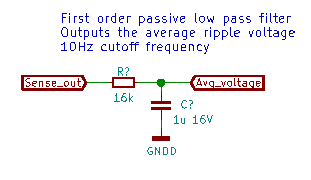
\includegraphics[width=0.35\textwidth]{current_sense/schematic/average_current.pdf}
    \end{center}
    \caption{Average current 10Hz cut-off low pass filter}
    \vspace{-22pt}
\end{wrapfigure}

To obtain the average inductor current ripple, the output of the previously designed current sense amplifier can be low pass filtered. By designing a first order passive low pass filter with a cut-off frequency of 10Hz, we can be sure to attenuate any selectable switching frequency by at least 40dB. This will provide a simple to measure DC voltage between 0.45V and 3V. This can be measured using the internal ADC of the ESP32 providing a theoretical resolution of 5mV, or 117$\mu$A. \todo{Please see} \Cref{A:specs} for the calculation of these values.


\subsection{Peak Inductor Current Sensing}\label{S:peak_current_design}

Based on the bandwidth requirement of 1kHz to 100kHz, it was identified that sampling the output signal of the current sensors to identify the peaks would be impractical. To achieve this a sampling rate of at least twice the highest frequency component would be specified by the Nyquist theorem, and a recommended minimum of one decade above is considered common practice, requiring a sampling rate of 1Mhz. 

Due to this, designs were undertaken to simplify the sampling requirements. The following designs will take direct input from the current sensor, and aim to output a DC voltage that is representative of the input current peak values. 

% discuss why it is that peak sensing is important, and how two designs have been created to achieve this task. The precision rectifier is my own design and not based on any existing designs, the sample and hold based sensor is based on designs from these resources \cite{peak_detector_designs, LTC6244_peak_detector}

\subsubsection*{Precision Rectifier Peak Voltage Detection}\label{S:current_sense_precision_rectifier_design}

This design is based around the operation of a signal precision rectifier, and the knowledge that the inductor current ripple will be symmetrical and triangular in shape \cite{Mohan2012_Design}. Due to this symmetry, we know that the average inductor ripple current over a period will be zero, shown in \Cref*{F:rectification} (a). After rectification of the signal, the the ripple peak to peak value will halve, the frequency will double, and the new signal average will be half the new ripple peak to peak, shown in \Cref*{F:rectification} (b). 

\begin{figure}[H]
    
    \centering
    \begin{subfigure}{0.49\textwidth}
        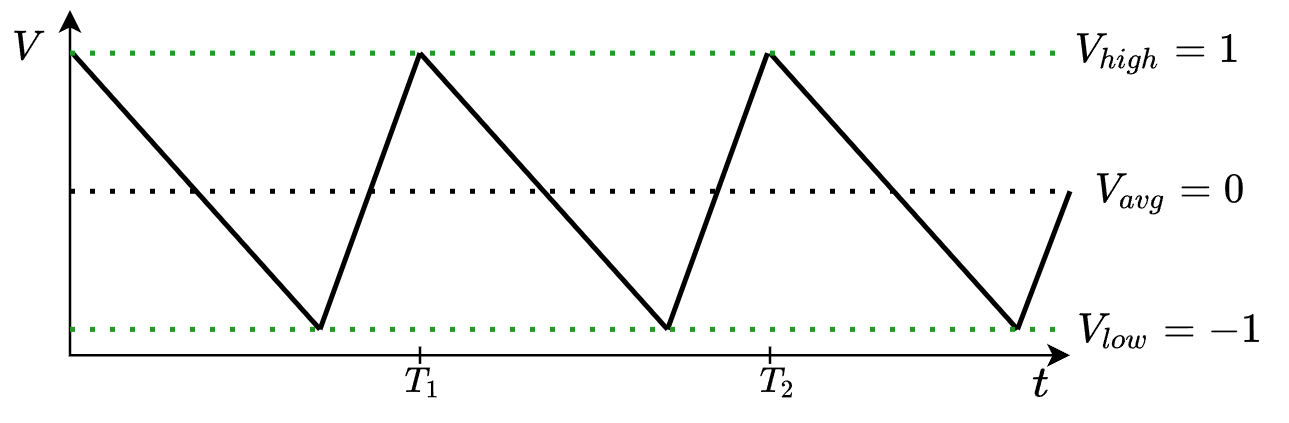
\includegraphics[width=\columnwidth]{current_sense/precision_rectification/pre_rectified.png}
        \subcaption{Pre-rectification current sense output of 1V pk to pk, average voltage of 0V}
    \end{subfigure}
    \begin{subfigure}{0.49\textwidth}
        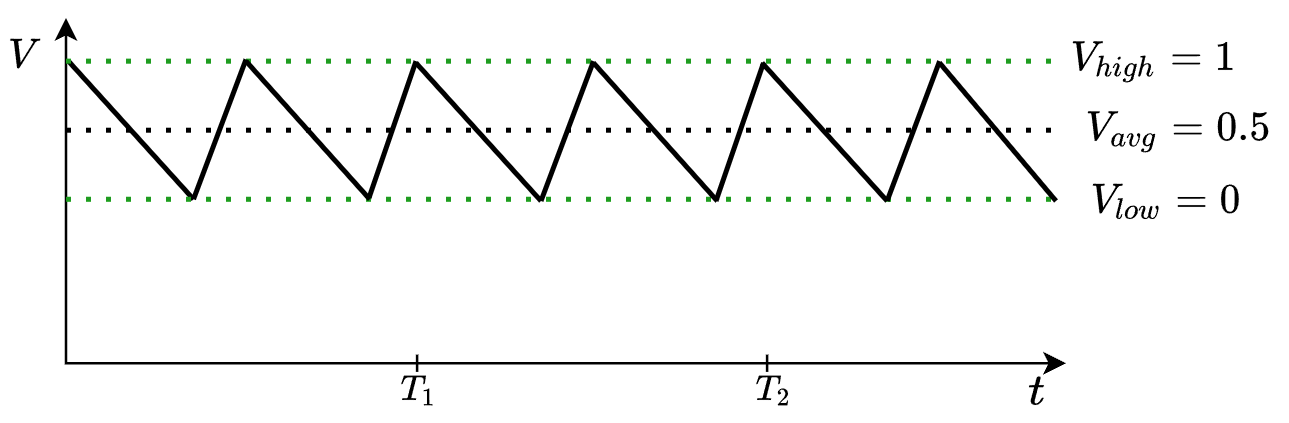
\includegraphics[width=\columnwidth]{current_sense/precision_rectification/post_rectified.png}
        \subcaption{Post-rectification current sense output of 1V pk to pk, average voltage of 0.5V}
    \end{subfigure}
    \caption{Average voltage output of a symmetrical signal, before and after rectification}
    \label{F:rectification}
\end{figure}

From here, we can obtain the signal average by applying a passive a low pass filter with a cut off of 10Hz to the output, producing a sampleable DC voltage. To obtain the full original signal peak to peak value, this signal can then amplified with a gain of 4. The full design can be seen in \Cref{F:precision_rectifier_circuit}.

\begin{figure}[!h]
    \centering
    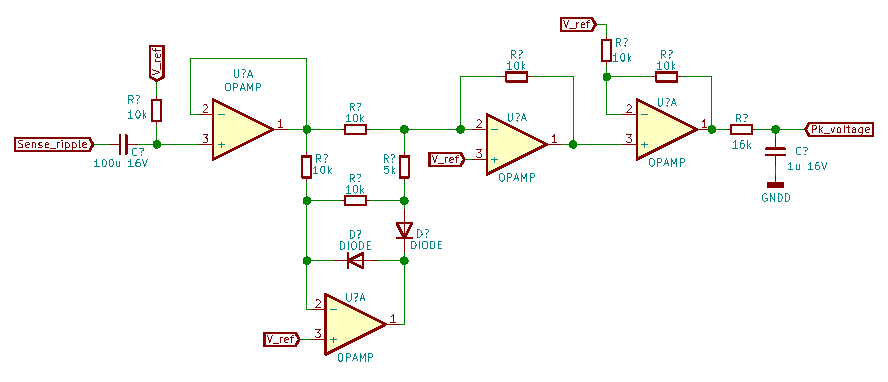
\includegraphics[width = 0.8\textwidth]{current_sense/schematic/precision_rectifier_schematic.pdf}
    \caption{Precision rectifier peak detector designed circuit schematic}
    \label{F:precision_rectifier_circuit}
\end{figure}

% Discuss the operation, and simulations of the Precision Rectifier Peak Voltage Detection. 

\subsubsection*{Sample and Hold Peak Voltage Detection}\label{S:current_sense_sample_and_hold_design}

This design is based on existing voltage peak detection designs \cite{peak_detector_designs,LTC6244_peak_detector}. The design operates on a similar principle to a sample and hold unit, charging a signal capturing capacitor through a diode such that it will not discharge. In order to remove the voltage drop across the charging diode, it is placed within the forward path of an operational amplifier buffer. The output voltage is then buffered again to allow for sampling. The full design can be seen in \Cref{F:sample_and_hold_circuit}.

\begin{figure}[!h]
    \centering
    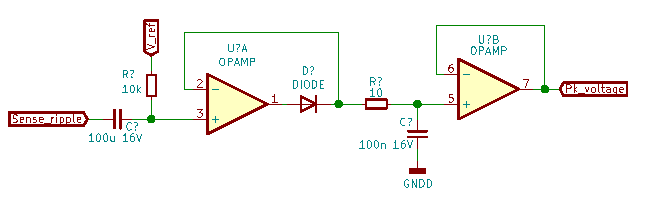
\includegraphics[width = 0.7\textwidth]{current_sense/schematic/sample_and_hold_schematic.pdf}
    \caption{Sample \& hold peak detector designed circuit schematic}
    \label{F:sample_and_hold_circuit}
\end{figure}

Both of the discussed designs have been simulated in LTSpice, and have had their operation confirmed, please see \Cref{A:peak_detector} for output plots. From this it was identified that both designs would be able to meet the resolution specification of 10mA, and bandwidth specification of 1kHz to 100kHz outlined in requirement 4, 5, 6, \& 7.

It should also be noted however that the design of the precision rectifier based peak detector is much more complex than that of the sample and hold peak detector. Because of this, it was decided that the sample and hold based peak detector would be most suitable for this project, as it meets all required specifications, and best adheres to the ease of use goal.


% Discuss the operation, and simulations of the Sample and Hold Peak Voltage Detection. Then discuss that due to it's simpler design, it's implementation will be far easier, the possible issue it may have will be easier to diagnose, and it's cost will be much lower. then specify that this was the final design selected for this section.

\subsection*{Current sensing digitisation}\label{S:current_sense_ADC_design}

Due to the operation of the design discussed in \Cref{S:current_sense_sample_and_hold_design}, the output DC voltage will be imposed on a DC refrence voltage. To eliminate this DC bias from the output, a dedicated external ADC with a differential input can be employed. This will allow for the removal of the bias at the digitisation of the signal. The selected ADC is the MAX11644, which provides a 12bit resolution, an internal reference of 4.096V, and the required differential input. 
Based on these specifications, this design is capable of measuring input voltages between 0V and 4.096V, with a resolution of 8mV. This will give a current sensing resolution of 2.6mA, meeting the specifications of requirement 6.


% Discuss the selection of the ADC for measuring the peak ripple and mean ripple currents. Talk about the minimum required ADC precision, and bandwidth requirements. Discuss hoe this AC provides a differential output. 


%
% SECTION Control System Design
%

\section{Control System}\label{S:control_design}

When designing the output voltage and inductor current ripple control systems, a successful design will meet all the requirements outlined by \Cref{S:specs_design}. From this we can identify that both controllers must provide a steady state error that is less $\pm$5\% of the targeted value, as specified in requirements 3 \& 6. 

\subsection{Output Load Voltage Controller}\label{S:output_control_design}

To achieve the desired output voltage steady state error, a feedback controller with an integrating term should be used. To provide this, the design will implement a proportional, integral, \& differential (PID) controller. This controller will be provided with the buck converter output voltage as an input, this will then be converted to the theoretical PWM duty cycle required to produce that output based on \Cref{E:V_out}. This will then be used to calculate the controller error and output the new PWM duty cycle.

To design this, a mathematical model of a buck converter \cite{Patil2015} was found and simulated in Matlab. This model was then discretised such that it could be implemented on a microcontroller, and a PID controller was then designed with the `\lstinline{PIDTune()}' function. A step response simulation of this model can be found in \Cref{A:control}. 

Due to the control topology used in this design, this design will be able to provide an output voltage steady state error of less than $\pm$5\%, as specified in requirement 3.

\subsection{Inductor Current Ripple Controller}\label{S:ripple_control_design}

To achieve the desired inductor current ripple steady state error, the same topology implemented for the output voltage controller will be implemented. This PID controller will take the system's inductor current ripple as a percentage of the average current, and then calculate the error between it and the target value. From here it will then output the new PWM switching frequency. 

Due to the control topology used in this design, this design will be able to provide an inductor current ripple steady state error of less than $\pm$5\%, as specified in requirement 6.




